\chapter{End-to-end example}
To illustrate the process documented in this thesis, we provide an end-to-end example on a small use case. This entails the process from modeling FPGAs all the way up to applying an emulation mapping on configurations of the virtual FPGA.

\section{FPGAs}
We introduce the virtual FPGA \textit{VirSample}. This simple FPGA has two inputs, has a 2-input-1-ouput LUT and two outputs (one of which is always zero). Figure \ref{fig:virsampleconfigs} shows the layout and different configurations of this virtual FPGA.

\begin{figure}
\centering
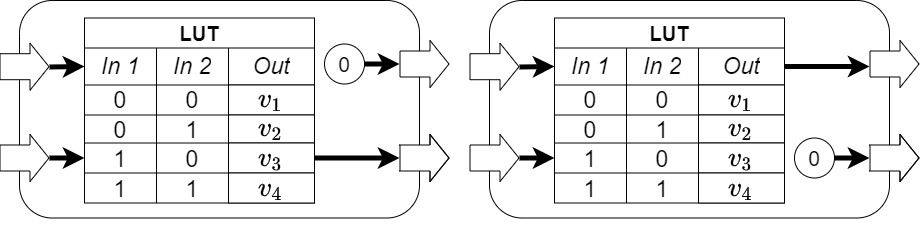
\includegraphics[width=0.8\textwidth]{images/endToEnd/exampleFPGA.png}
\caption{Both configurations of VirSample. The left configuration is specified by configuration bit $v_5=0$ while the right configuration is specified by $v_5=1$.}
\label{fig:visampleconfigs}
\end{figure}

Suppose we want to emulate configurations of VirSample on a real, physical FPGA ConcreteSample (shown in Figure \ref{fig:conboardconfigs}). This FPGA has a 2-input-2-output logic cell, a register and a multiplexer (a component that selects one of its two input sets as output depending on its configuration). Intuitively, we may find an emulation mapping by hand:

\begin{minipage}{\textwidth}
\begin{itemize}
\item $c_1 \longleftarrow v_5 \land v_1$
\item $c_2 \longleftarrow \lnot v_5 \land v_1$
\item $c_3 \longleftarrow v_5 \land v_2$
\item $c_4 \longleftarrow \lnot v_5 \land v_1$
\item $c_5 \longleftarrow v_5 \land v_3$
\item $c_6 \longleftarrow \lnot v_5 \land v_3$
\item $c_7 \longleftarrow v_5 \land v_4$
\item $c_8 \longleftarrow \lnot v_5 \land v_4$
\item $c_9 \longleftarrow 0$
\item virtual input 1 $=$ concrete input 1
\item virtual input 2 $=$ concrete input 2
\item virtual output 1 $=$ concrete output 1
\item virtual output 2 $=$ concrete output 3
\end{itemize}
\end{minipage}

We will show that a similar emulation mapping will also be the result of applying our method. First, we will design graph models for both FPGAs in Section \ref{sec:example-graphmodels}. We will find a subgraph homeomorphism between those graphs in Section \ref{sec:example-subiso}. Finally, we will retrieve the emulation mapping in Section \ref{sec:example-obtainingemulation}.

	

\begin{figure}[t]
\centering
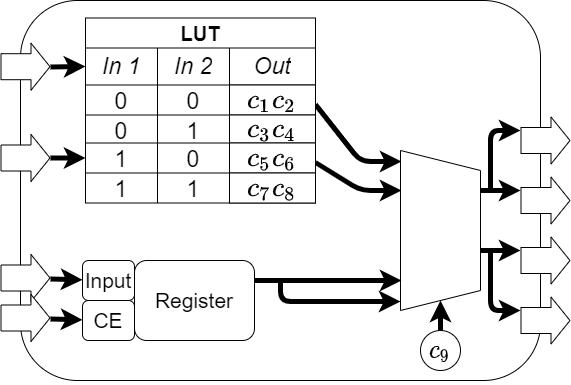
\includegraphics[width=0.5\textwidth]{images/endToEnd/exampleFPGAConcrete.png}
\caption{The ConcreteSample FPGA. It has 9 configurable bits, 8 of which in its lookup table and one of which a selector of its multiplexer.}
\label{fig:conboardconfigs}
\end{figure}



\section{Graph models}
\label{sec:example-graphmodels}
We model our FPGAs using the model specified in Chapter \ref{chapter:models}, with one addition: we model LUTs with a new label \texttt{LOGIC}. Since we only model physical structures (i.e. wires, transistors and logical components) instead of semantics, we need to think of ways that VirSample could have been implemented using these physical structures. After all, this FPGA does not physically exist. Some implementations of VirSample will yield graph models that have subgraph homeomorphism embeddings in ConcreteSample's graph while some will not. In this example, we will make a single compact graph model, although for practical use we recommend trying out different models. This graph model is shown in Figure \ref{fig:example-virtualGraph}. This model assumes that the physical implementation of VirSample uses a 2-input-2-output LUT, with the limitation that for each input combination in the LUT, at least one output should be configured to be zero, depending on $v_5$.

\begin{figure}[t]
\centering
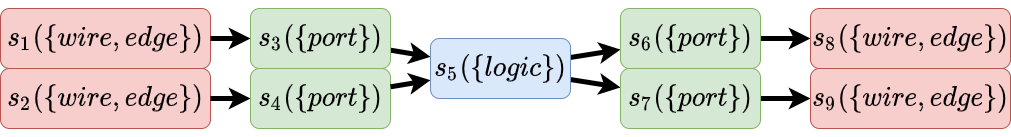
\includegraphics[width=0.8\textwidth]{images/endToEnd/virtualFPGAGraph.png}
\caption{Graph model of the virtual FPGA.}
\label{fig:example-virtualGraph}
\end{figure}

Obtaining the graph model for the concrete FPGA is easier: since ConcreteSample physically exists, we already know where transistors, wires and LUTs are used. Using the model from Chapter \ref{chapter:models} with the LUT addition we obtain the graph shown in Figure \ref{fig:example-concreteGraph}. We omit the register since we logically induce that, since VirSample only uses combinatorial components, an emulation on ConcreteSample would never include usage of its register.

\begin{figure}[h]
\centering
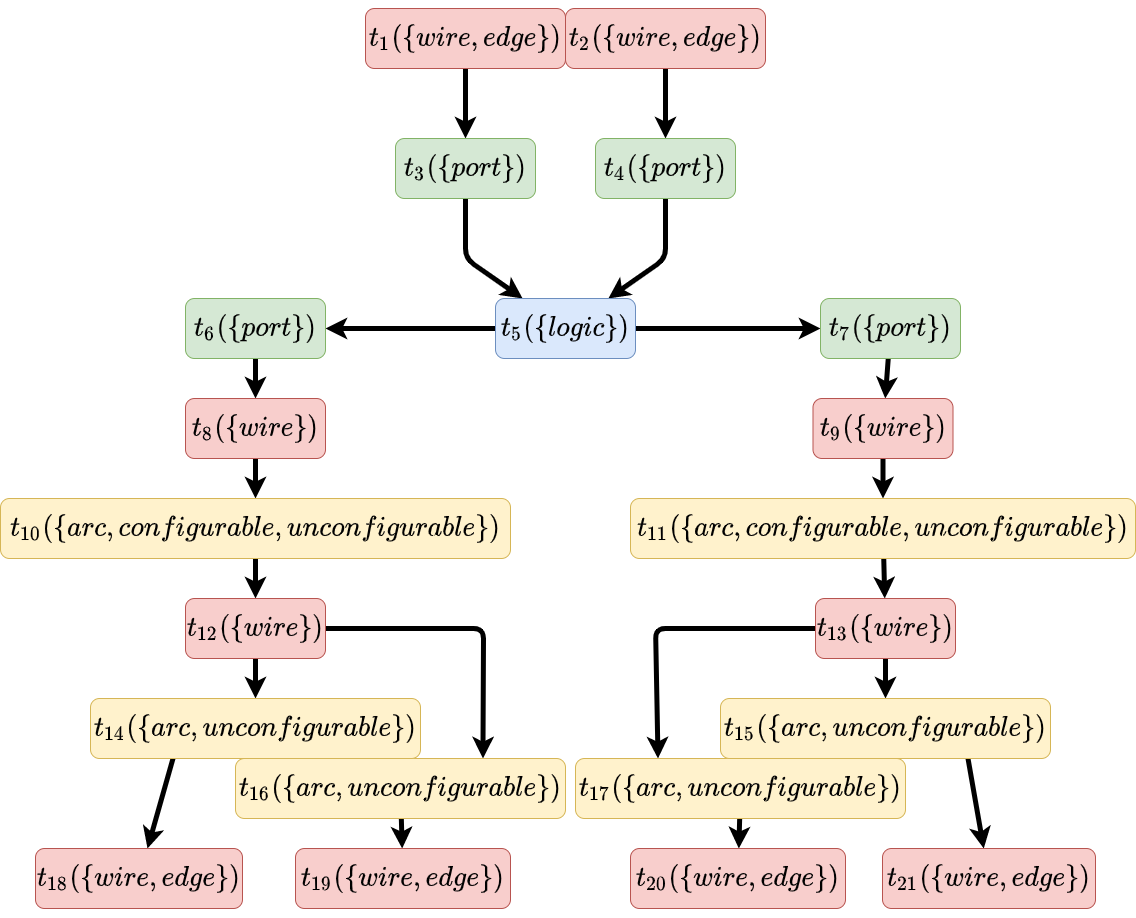
\includegraphics[width=0.8\textwidth]{images/endToEnd/concreteFPGAGraph.png}
\caption{Graph model of the concrete FPGA.}
\label{fig:example-concreteGraph}
\end{figure}	


\section{Finding a subgraph homeomorphism}
\subsection{Applying ordering}
We apply GreatestConstrainedFirst to our source graph from Figure \ref{fig:example-virtualGraph} to obtain the graph shown in Figure \ref{fig:example-virtualGraphOrdered}.

\begin{figure}
\centering
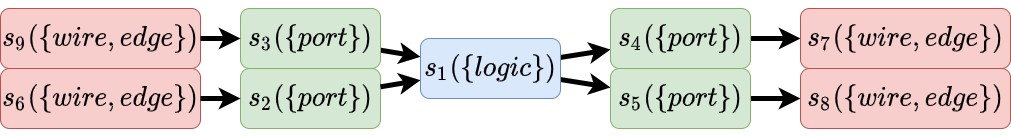
\includegraphics[width=0.8\textwidth]{images/endToEnd/virtualFPGAGraphOrdered.png}
\caption{Graph model of the virtual FPGA with vertices ordered using GreatestConstrainedFirst.}
\label{fig:example-virtualGraphOrdered}
\end{figure}

Furthermore, we order the target graph vertices from the target graph from Figure \ref{fig:example-concreteGraph}
by degree to obtain the graph shown in Figure \ref{fig:example-virtualGraphOrdered}

\begin{figure}[h]
\centering
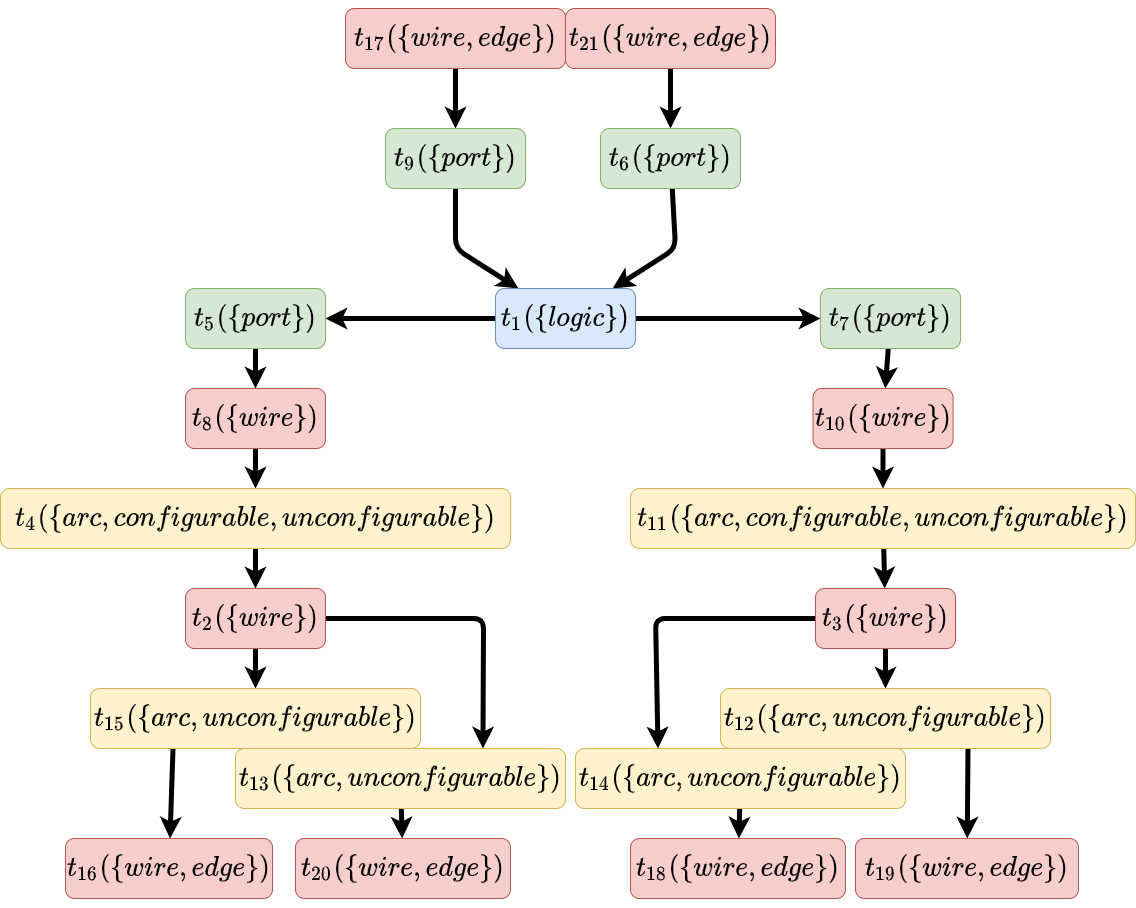
\includegraphics[width=0.8\textwidth]{images/endToEnd/concreteFPGAGraphOrdered.png}
\caption{Graph model of the concrete FPGA with vertices ordered by degree.}
\label{fig:example-concreteGraphOrdered}
\end{figure}


\label{sec:example-subiso}
\subsection{Applying contraction}
We use our algorithm with contraction enabled, meaning we will  preprocess our source graph to reduce its size, keeping track of contracted vertices to use later in the algorithm. Contracting each source graph vertex with indegree 1 and outdegree 1 leaves us with the graph shown in Figure \ref{fig:example-virtualGraphContracted}.

\begin{figure}[h]
\centering
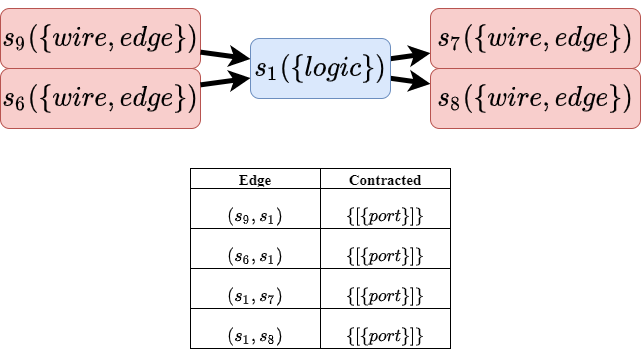
\includegraphics[width=0.5\textwidth]{images/endToEnd/exampleFPGAContracted.png}
\caption{Contracted graph model of the virtual FPGA.}
\label{fig:example-virtualGraphContracted}
\end{figure}

\subsection{Running algorithm}
We start with a partial mapping $(\mathit{vmap}, \mathit{emap})$ where $\mathit{vmap}$ and $\mathit{emap}$ are both empty and run Algorithm \ref{algorithm:ndSHD2-ext}.

\begin{longtable}{llp{15cm}}
\bullet & (lines \ref{line:ifHasUnmatchedEdge}, \ref{line:getNextVertexPair}) & There exists no unmatched edge, so retrieve the next node pair $(s_1, t_1)$. \\

\bullet & (line \ref{line:pruneVertex})     & The pruner (which uses N-reachability filtering) obtains the domains: \newline $s_1 \to \{t_1\}$ \newline $ s_6 \to \{t_{17}, t_{21}\}$\newline$s_7 \to \{t_{16}, t_{18}, t_{19}, t_{20}\}$\newline$s_8 \to \{t_{16}, t_{18}, t_{19}, t_{20}\}$\newline$s_9 \to \{t_{17}, t_{21}\}$ \newline Since an injective mapping exists from this domain, we do not prune.  \\

\bullet & (line \ref{line:addToVmap}) & We add $(s_1, t_1)$ to $\mathit{vmap}$, which is now $\{(s_1, t_1)\}$. \\ 

\bullet & (line \ref{line:recursiveVertex}) & We enter a recursive call. \\ 

\bullet & (lines \ref{line:ifHasUnmatchedEdge}, \ref{line:getNextVertexPair}) & There exists no unmatched edge, so retrieve the next node pair. For briefness, we will omit attempts to match $s_6$ with $t_1 \dots t_{16}$: these will each result in being pruned in line 11 because of reachability and label compatibility problems, until we try $(s_6, t_{17})$. \\ 

\bullet & (line \ref{line:pruneVertex}) & The pruner (which uses N-reachability filtering) obtains the domains: \newline $s_1 \to \{t_1\}$ \newline $s_6 \to \{t_{17}\}$ \newline $s_7 \to \{t_{16}, t_{18}, t_{19}, t_{20}\}$ \newline $s_8 \to \{t_{16}, t_{18}, t_{19}, t_{20}\}$ \newline $s_9 \to \{t_{21}\}$ \newline Since an injective mapping exists from this domain, we do not prune.\\ 

\bullet & (line \ref{line:addToVmap}) & We add $(s_6, t_{17})$ to $\mathit{vmap}$, which is now $\{(s_1, t_1), (s_6, t_{17}))\}$.\\ 

\bullet & (line \ref{line:recursiveVertex}) & We enter a recursive call.\\ 

\bullet & (lines \ref{line:ifHasUnmatchedEdge}, \ref{line:getNextEdgePathPair}) & There exists an unmatched edge $(s_6, s_1)$, so retrieve the next edge-path pair (using DFS path iteration) $(s_6\to s_1, t_{17} \to t_9 \to t_1)$.\\ 

\bullet & (line \ref{line:unneccesarilyLong}) & Since no shortcuts exist in the path $t_{17} \to t_9 \to t_1$, $\mathit{isUnnecessarilyLong}(t_{17} \to t_9 \to t_1)$ is false.\\ 

\bullet & (line \ref{line:prunePath}) & The pruner (which uses N-reachability filtering) obtains the domains: \newline $s_1 \to \{t_1\}$ \newline $ s_6 \to \{t_{17}\}$ \newline $s_7 \to \{t_{16}, t_{18}, t_{19}, t_{20}\}$ \newline $s_8 \to \{t_{16}, t_{18}, t_{19}, t_{20}\}$ \newline $ s_9 \to \{t_{21}\}$ \newline Since an injective mapping exists from this domain, we do not prune.\\ 

\bullet & (line \ref{line:contractionCheck}) & Contraction is enabled, and we find that the path $t_{17} \to t_9 \to t_1$ satisfies the requirements of having a single intermediate vertex with at least the label \texttt{PORT} (vertex $t_9$). Therefore, we do not prune.\\ 

\bullet & (line \ref{line:addToEmap}) & We add $(s_6\to s_1, t_{17} \to t_9 \to t_1)$ to $\mathit{emap}$, which is now $\{(s_6\to s_1, t_{17} \to t_9 \to t_1)\}$.\\ 

\bullet & (line \ref{line:recursivePath}) & We enter a recursive call.\\ 

\bullet & (lines \ref{line:ifHasUnmatchedEdge}, \ref{line:getNextVertexPair}) & There exists no unmatched edge, so retrieve the next node pair $(s_7, t_{16})$. For briefness, we will omit attempts to match $s_7$ with $t_1 \dots t_{15}$: these will each result in being pruned in line 11 because of reachability and label compatibility problems, until we try $(s_7, t_{16})$.\\ 

\bullet & (line \ref{line:pruneVertex}) & The pruner (which uses N-reachability filtering) obtains the domains: \newline $s_1 \to \{t_1\}$ \newline $s_6 \to \{t_{17}\}$ \newline $s_7 \to \{t_{16}\}$ \newline $s_8 \to \{t_{18}, t_{19}, t_{20}\}$ \newline $s_9 \to \{t_{21}\}$ \newline Since an injective mapping exists from this domain, we do not prune. \\ 

\bullet & (line \ref{line:addToVmap}) & We add $(s_7, t_{16})$ to $\mathit{vmap}$, which is now $\{(s_1, t_1), (s_6, t_{17}), (s_7, t_{16}))\}$.\\ 

\bullet & (line \ref{line:recursiveVertex}) & We enter a recursive call.\\ 

\bullet & (lines \ref{line:ifHasUnmatchedEdge}, \ref{line:getNextEdgePathPair}) & There exists an unmatched edge $(s_1, s_7)$, so retrieve the next edge-path pair (using DFS path iteration) $(s_1\to s_7, t_1 \to t_5 \to t_8 \to t_4 \to t_2 \to t_{15} \to t_{16})$.\\ 

\bullet & (line \ref{line:unneccesarilyLong}) & Since no shortcuts exist in the path $t_1 \to t_5 \to t_8 \to t_4 \to t_2 \to t_{15} \to t_{16}$, $\mathit{isUnnecessarilyLong}(t_1 \to t_5 \to t_8 \to t_4 \to t_2 \to t_{15} \to t_{16})$ is false.\\ 

\bullet & (line \ref{line:prunePath}) & The pruner (which uses N-reachability filtering) obtains the domains: \newline $s_1 \to \{t_1\}$ \newline $s_6 \to \{t_{17}\}$ \newline $s_7 \to \{t_{16}\}$ \newline  $s_8 \to \{t_{18}, t_{19}\}$ \newline $s_9 \to \{t_{21}\}$ \newline Since an injective mapping exists from this domain, we do not prune.\\ 

\bullet & (line \ref{line:contractionCheck}) & Contraction is enabled, and we find that the path $t_1 \to t_5 \to t_8 \to t_4 \to t_2 \to t_{15} \to t_{16}$ satisfies the requirements of having a single intermediate vertex with at least the label \texttt{PORT} (vertex $t_5$). Therefore, we do not prune.\\ 

\bullet & (line \ref{line:removeFromCoverPath}) & Since vertex $t_{20}$ is in the cover reachable by vertices from this path through unconfigurable transistors, we delete it from the graph until this path is backtracked.\\ 

\bullet & (line \ref{line:addToEmap}) & We add $(s_1\to s_7, t_1 \to t_5 \to t_8 \to t_4 \to t_2 \to t_{15} \to t_{16})$ to $\mathit{emap}$, which is now $\{(s_6\to s_1, t_{17} \to t_9 \to t_1), (s_1\to s_7, t_1 \to t_5 \to t_8 \to t_4 \to t_2 \to t_{15} \to t_{16})\}$.\\ 

\bullet & (line \ref{line:recursivePath}) & We enter a recursive call.\\ 

\bullet & (lines \ref{line:ifHasUnmatchedEdge}, \ref{line:getNextVertexPair}) & There exists no unmatched edge, so retrieve the next node pair $(s_8, t_{18})$. For briefness, we will omit attempts to match $s_7$ with $t_1 \dots t_{17}$: these will each result in being pruned in line 11 because of reachability and label compatibility problems, until we try $(s_8, t_{18})$.\\ 

\bullet & (line \ref{line:pruneVertex}) & The pruner (which uses N-reachability filtering) obtains the domains: \newline $s_1 \to \{t_1\}$ \newline $s_6 \to \{t_{17}\}$ \newline $s_7 \to \{t_{16}\}$ \newline $s_8 \to \{t_{18}\}$ \newline $s_9 \to \{t_{21}\}$ \newline Since an injective mapping exists from this domain, we do not prune.\\ 

\bullet & (line \ref{line:addToVmap}) & We add $(s_8, t_{18})$ to $\mathit{vmap}$, which is now $\{(s_1, t_1), (s_6, t_{17}), (s_7, t_{16}), (s_8, t_{18})\}$.\\ 

\bullet & (line \ref{line:recursiveVertex}) & We enter a recursive call.\\ 

\bullet & (lines \ref{line:ifHasUnmatchedEdge}, \ref{line:getNextEdgePathPair}) & There exists an unmatched edge $(s_1, s_8)$, so retrieve the next edge-path pair (using DFS path iteration) $(s_1\to s_8, t_1 \to t_7 \to t_{10} \to t_{11} \to t_3 \to t_{14} \to t_{18})$.\\ 

\bullet & (line \ref{line:unneccesarilyLong}) & Since no shortcuts exist in the path {$t_1 \to t_7 \to t_{10} \to t_{11} \to t_3 \to t_{14} \to t_{18}$}, $\mathit{isUnnecessarilyLong}(t_1 \to t_7 \to t_{10} \to t_{11} \to t_3 \to t_{14} \to t_{18})$ is false.\\ 

\bullet & (line \ref{line:prunePath}) & The pruner (which uses N-reachability filtering) obtains the domains: \newline $s_1 \to \{t_1\}$ \newline $s_6 \to \{t_{17}\}$ \newline $s_7 \to \{t_{16}\}$ \newline $s_8 \to \{t_{18}\}$ \newline $s_9 \to \{t_{21}\}$ \newline Since an injective mapping exists from this domain, we do not prune.\\ 

\bullet & (line \ref{line:contractionCheck}) & Contraction is enabled, and we find that the path $t_1 \to t_7 \to t_{10} \to t_{11} \to t_3 \to t_{14} \to t_{18}$ satisfies the requirements of having a single intermediate vertex with at least the label \texttt{PORT} (vertex $t_7$). Therefore, we do not prune.\\ 

\bullet & (line \ref{line:removeFromCoverPath}) & Since vertex $t_{19}$ is in the cover reachable by vertices from this path through unconfigurable transistors, we delete it from the graph until this path is backtracked.\\ 

\bullet & (line \ref{line:addToEmap}) & We add $(s_1\to s_7, t_1 \to t_5 \to t_8 \to t_4 \to t_2 \to t_{15} \to t_{16})$ to $\mathit{emap}$, which is now:\newline $\{(s_6\to s_1, t_{17} \to t_9 \to t_1),$\newline$(s_1\to s_7, t_1 \to t_5 \to t_8 \to t_4 \to t_2 \to t_{15} \to t_{16}),$\newline$(s_1 \to s_8, t_1 \to t_7 \to t_{10} \to t_{11} \to t_3 \to t_{14} \to t_{18})\}$.\\ 

\bullet & (line \ref{line:recursivePath}) & We enter a recursive call.\\ 

\bullet & (lines \ref{line:ifHasUnmatchedEdge}, \ref{line:getNextVertexPair}) & There exists no unmatched edge, so retrieve the next node pair. For briefness, we will omit attempts to match $s_6$ with $t_1 \dots t_{20}$: these will each result in being pruned in line 11 because of reachability and label compatibility problems, until we try $(s_9, t_{21})$.\\ 

\bullet & (line \ref{line:pruneVertex}) & The pruner (which uses N-reachability filtering) obtains the domains: \newline $s_1 \to \{t_1\}$ \newline $s_6 \to \{t_{17}\}$ \newline $s_7 \to \{t_{16}\}$ \newline $s_8 \to \{t_{18}\}$ \newline $s_9 \to \{t_{21}\}$ \newline Since an injective mapping exists from this domain, we do not prune.\\ 


\bullet & (line \ref{line:addToVmap}) & We add $(s_9, t_{21})$ to $\mathit{vmap}$, which is now $\{(s_1, t_1), (s_6, t_{17}), (s_7, t_{16}), (s_8, t_{18}), (s_9, t_{21})\}$.\\ 

\bullet & (line \ref{line:recursiveVertex}) & We enter a recursive call.\\ 

\bullet & (lines \ref{line:ifHasUnmatchedEdge}, \ref{line:getNextEdgePathPair}) & There exists an unmatched edge $(s_{9}, s_1)$, so retrieve the next edge-path pair (using DFS path iteration) $(s_9 \to s_1, t_{21} \to t_6 \to t_1)$.\\ 

\bullet & (line \ref{line:unneccesarilyLong}) & Since no shortcuts exist in the path $t_{21} \to t_6 \to t_1$, $\mathit{isUnnecessarilyLong}(t_{21} \to t_6 \to t_1)$ is false.\\ 

\bullet & (line \ref{line:prunePath}) & The pruner (which uses N-reachability filtering) obtains the domains: \newline $s_1 \to \{t_1\}$ \newline $s_6 \to \{t_{17}\}$ \newline $s_7 \to \{t_{16}\}$ \newline $s_8 \to \{t_{18}\}$ \newline $s_9 \to \{t_{21}\}$ \newline Since an injective mapping exists from this domain, we do not prune.\\ 

\bullet & (line \ref{line:contractionCheck}) & Contraction is enabled, and we find that the path $t_{21} \to t_6 \to t_1$ satisfies the requirements of having a single intermediate vertex with at least the label \texttt{PORT} (vertex $t_6$). Therefore, we do not prune.\\ 

\bullet & (line \ref{line:addToEmap}) & We add $(s_9 \to s_1, t_{21} \to t_6 \to t_1)$ to $\mathit{emap}$, which is now:\newline $\{(s_6\to s_1, t_{17} \to t_9 \to t_1),$\newline$(s_1\to s_7, t_1 \to t_5 \to t_8 \to t_4 \to t_2 \to t_{15} \to t_{16}),$\newline$(s_1 \to s_8, t_1 \to t_7 \to t_{10} \to t_{11} \to t_3 \to t_{14} \to t_{18}),$\newline$(s_9 \to s_1, t_{21} \to t_6 \to t_1)\}$.\\ 


\bullet & (line \ref{line:recursivePath}) & We enter a recursive call.\\ 

\bullet & (line \ref{line:returnTrueFirstTime}) & Since the partial mapping is complete, we return true.\\ 

\bullet & (line \ref{line:returnRecursivePath}) & We return true from the recursive call, along with $(\mathit{vmap}, \mathit{emap})$\\ 

\bullet & (line \ref{line:returnRecursiveVertex}) & We return true from the recursive call, along with $(\mathit{vmap}, \mathit{emap})$\\

\bullet & (line \ref{line:returnRecursivePath}) & We return true from the recursive call, along with $(\mathit{vmap}, \mathit{emap})$\\ 

\bullet & (line \ref{line:returnRecursiveVertex}) & We return true from the recursive call, along with $(\mathit{vmap}, \mathit{emap})$\\ 

\bullet & (line \ref{line:returnRecursivePath}) & We return true from the recursive call, along with $(\mathit{vmap}, \mathit{emap})$\\ 

\bullet & (line \ref{line:returnRecursiveVertex}) & We return true from the recursive call, along with $(\mathit{vmap}, \mathit{emap})$\\

\bullet & (line \ref{line:returnRecursivePath}) & We return true from the recursive call, along with $(\mathit{vmap}, \mathit{emap})$\\ 

\bullet & (line \ref{line:returnRecursiveVertex}) & We return true from the recursive call, along with $(\mathit{vmap}, \mathit{emap})$\\ 

\bullet & (line \ref{line:returnRecursiveVertex}) & We return true from the recursive call, along with $(\mathit{vmap}, \mathit{emap})$\\ 
\end{longtable}

In the end, we have a subgraph homeomorphism with the vertex-on-vertex mapping:

$\{(s_1, t_1), (s_6, t_{17}), (s_7, t_{16}), (s_8, t_{18}), (s_9, t_{21})\}$

and the following edge-on-path mapping:


$\{(s_6\to s_1, t_{17} \to t_9 \to t_1),$ \newline
$(s_1\to s_7,t_1 \to t_5 \to t_8 \to t_4 \to t_2 \to t_{15} \to t_{16}),$\newline
$(s_1\to s_8,t_1 \to t_7 \to t_{10} \to t_{11} \to t_3 \to t_{14} \to t_{18}),$\newline
$(s_9 \to s_1, t_{21} \to t_6 \to t_1)\}$

\section{Obtaining emulation mapping}
\label{sec:example-obtainingemulation}

To obtain the emulation mapping, we follow the following rules:
\begin{enumerate}
\item For each contracted vertex replaced by some edge $e$, assume that is is matched with the first label-compatible vertex in the path $M(e)$.
\item Each configurable concrete FPGA transistor that is not in the subgraph homeomorphism is configured to be disabled (i.e. does not allow an electrical current to flow through them).
\item Each configurable concrete FPGA transistor $M(s)$ that is in the subgraph homeomorphism in the vertex-vertex mapping is configured equal to transistor $s$.
\item Each configurable concrete FPGA transistor that is in the subgraph homeomorphism in the edge-path mapping as intermediate vertex is configured to be enabled, i.e. always letting electrical current flow through.
\item Each concrete FPGA LUT that is not in not the subgraph homeomorphism is configured to output all zeroes regardless of the input.
\item Each concrete FPGA LUT that is in the subgraph homeomorphism as part of the vertex-vertex mapping is configured based on the configuration of the virtual LUT such that if the input \texttt{PORT} vertices of the virtual FPGA graph $\mathit{s\mhyphen in}_1 \dots \mathit{s\mhyphen in}_m$ are mapped to concrete FPGA vertices $\mathit{t\mhyphen in}_1 \dots \mathit{t\mhyphen in}_m$ and the output \texttt{PORT} vertices of the virtual FPGA graph $\mathit{s\mhyphen out}_1 \dots \mathit{s\mhyphen out}_n$ are mapped to concrete FPGA vertices $\mathit{t\mhyphen out}_1 \dots \mathit{t\mhyphen out}_n$, the function implemented by the concrete FPGA LUT from $\mathit{t\mhyphen in}_1 \dots \mathit{t\mhyphen in}_m$ to $\mathit{t\mhyphen out}_1 \dots \mathit{t\mhyphen out}_n$ is equal to the function implemented from $\mathit{s\mhyphen in}_1 \dots \mathit{s\mhyphen in}_m$ to $\mathit{s\mhyphen out}_1 \dots \mathit{s\mhyphen out}_n$. All remaining outputs should be configured to be zero.
\item Each concrete FPGA LUT that is is in the subgraph homeomorphism in the edge-path mapping as intermediate vertex is configured to output the value of its one input that is in the mapping to its one output that is in the mapping, and zeroes to each other output.
\item To emulate a signal coming into the virtual FPGA on some input wire $s$, one should send the same signal to the input wire $M(s)$ on the concrete FPGA.
\item The emulated output of each virtual FPGA output wire $s$ is the output of the concrete FPGA output wire $M(s)$.
\end{enumerate}


Following these rules and the obtained subgraph homeomorphism, we establish the following configuration mapping:

\begin{itemize}
\item $c_1 \longleftarrow v_5 \land v_1$
\item $c_2 \longleftarrow \lnot v_5 \land v_1$
\item $c_3 \longleftarrow v_5 \land v_2$
\item $c_4 \longleftarrow \lnot v_5 \land v_1$
\item $c_5 \longleftarrow v_5 \land v_3$
\item $c_6 \longleftarrow \lnot v_5 \land v_3$
\item $c_7 \longleftarrow v_5 \land v_4$
\item $c_8 \longleftarrow \lnot v_5 \land v_4$
\item $c_9 \longleftarrow 0$
\item virtual input 1 $=$ concrete input 1
\item virtual input 2 $=$ concrete input 2
\item virtual output 1 $=$ concrete output 2
\item virtual output 2 $=$ concrete output 4
\end{itemize}

Now, whenever a student creates a configuration consisting of values $v_1 \dots v_5$ for the virtual FPGA, a configuration is also defined by the values $c_1 \dots c_9$ for the concrete FPGA that has the same semantics.

